\documentclass[11pt]{extarticle}
\usepackage{manualdoprofessor}
\usepackage{fichatecnica}
\usepackage{lipsum,media9}
\usepackage[justification=raggedright]{caption}
\usepackage[one]{bncc}
\usepackage[acorde]{../edlab}
\usepackage{marginnote}
\usepackage{pdfpages}
\usepackage[printwatermark]{xwatermark}
%\newwatermark[pagex=2]{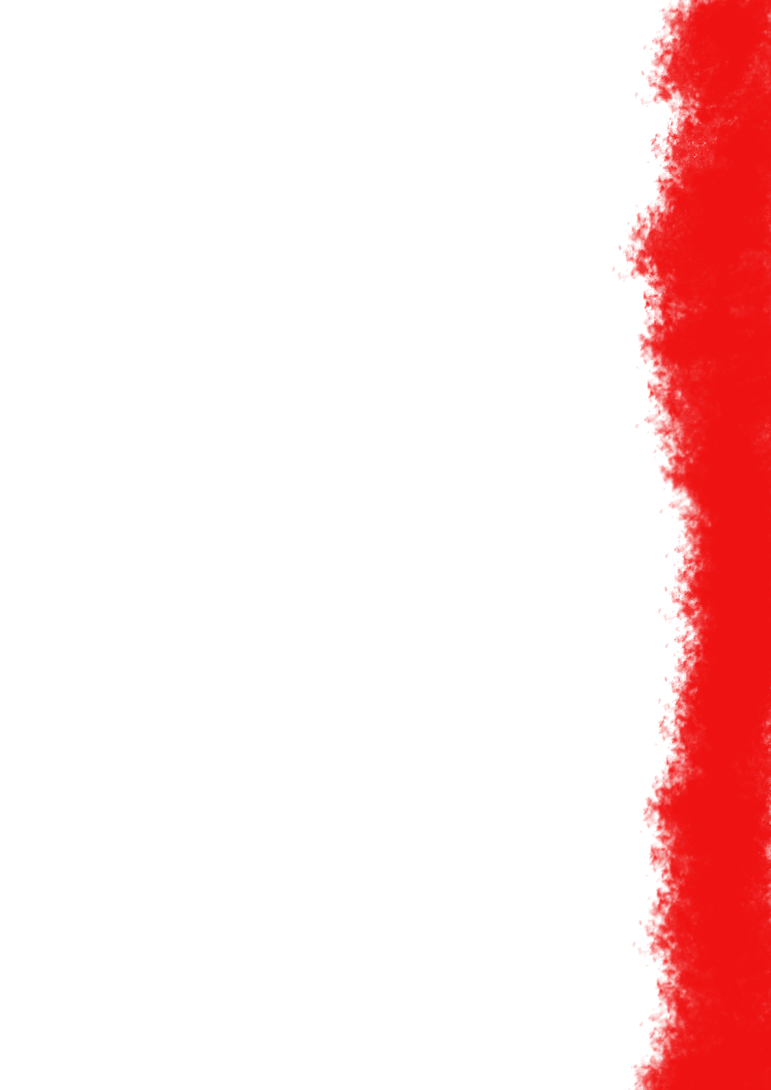
\includegraphics[scale=3.3]{watermarks/test-a.png}}	% página específica
%\newwatermark[oddpages]{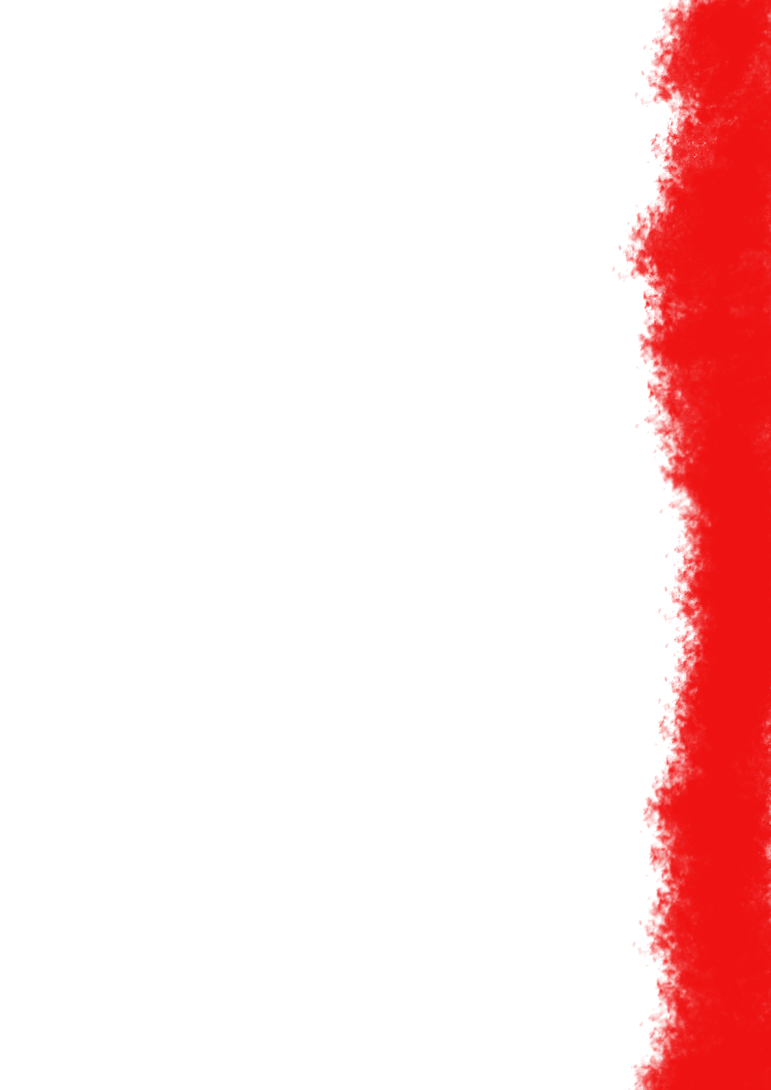
\includegraphics{watermarks/test-a.png}}			% páginas ímpars
%\newwatermark[evenpages]{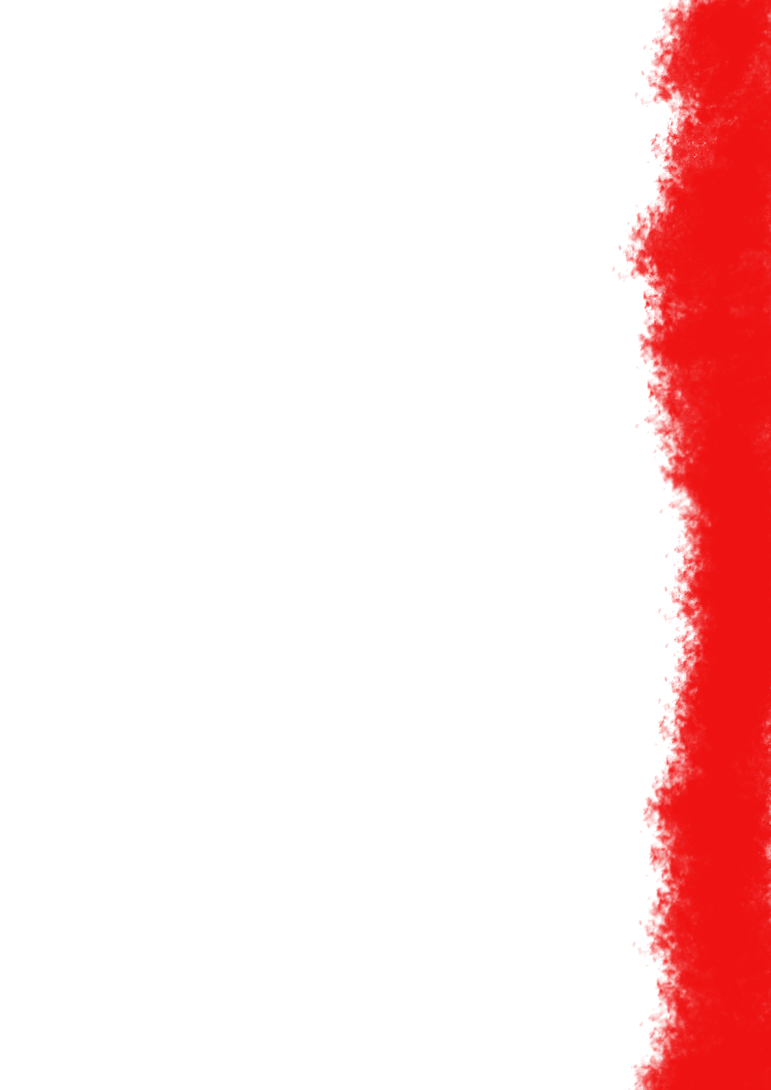
\includegraphics{watermarks/test-a.png}}			% págimas pares
%\newwatermark[allpages]{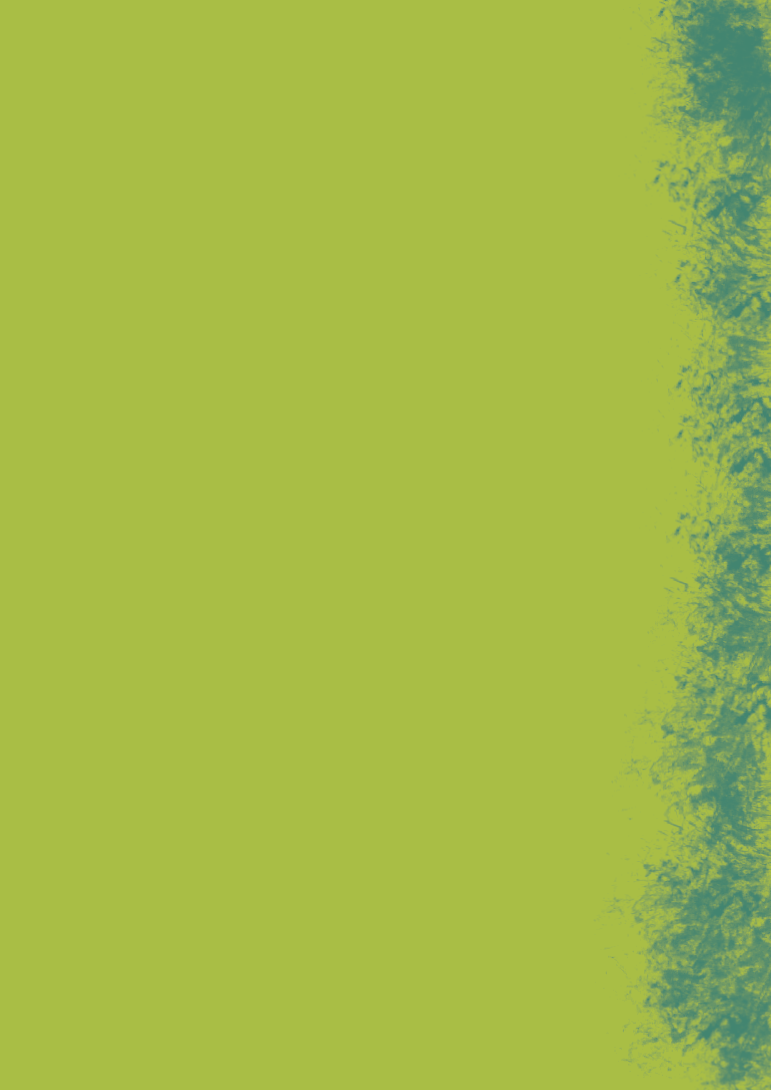
\includegraphics[scale=3.3]{watermarks/test-b.png}}
%\pagecolor{cyan!0!magenta!10!yellow!28!black!28!}

\newcommand{\AutorLivro}{Bruna Martins}
\newcommand{\TituloLivro}{Onde moram as coisas}
\newcommand{\Genero}{Memória literária}
%\newcommand{\imagemCapa}{./images/PNLD0001-01.png}
\newcommand{\issnppub}{978-65-99441-24-0}
\newcommand{\issnepub}{978-65-99441-27-1}
% \newcommand{\fichacatalografica}{PNLD0001-00.png}
\newcommand{\colaborador}{Gabriela Karam}

\begin{document}

\title{\TituloLivro}
\author{\AutorLivro}
\def\authornotes{\colaborador}

\date{}
\maketitle

%\begin{abstract}\addcontentsline{toc}{section}{Carta ao professor}
%\pagebreak

\tableofcontents


\begin{abstract}
Caras e caros educadores,

Este material tem a intenção de contribuir para que vocês desenvolvam um trabalho aprofundado com a obra \textit{Onde moram as coisas} em sala de aula.
Vocês encontrarão informações sobre o autor, sobre o gênero e também 
algumas propostas de trabalho para a sala de aula que poderão ser exploradas livremente, 
da forma que vocês considerarem mais apropriadas para os seus estudantes. Contamos com vocês para mergulharmos juntos nessa história cheia de objetos antigos, cheiros, texturas e emoções como se fizéssemos uma visita ao apartamento de Dona Pedrina, a avó da autora Bruna Martins. 

O livro é o trabalho de conclusão de curso de Bruna, que estudou na Faculdade de Arquitetura e Urbanismo da Universidade de São Paulo e terminou o curso em 2021. A autora decidiu fazer um percurso ilustrado pela casa da avó, revisitando seus cômodos e objetos através das memórias afetivas que as duas guardam daqueles espaços. 

Alguns objetos e espaços físicos podem nos transportar para lugares longínquos da nossa realidade e fazer relações com emoções profundas que guardamos e muitas vezes nem temos conhecimento de que existiam. O educador, filósofo e psicanalista Rubem Alves, em uma de suas crônicas, faz a seguinte citação:

\begin{quote}

``Existe sempre a fantasia de que, num momento futuro, será possível criar uma máquina que nos permita viajar através do tempo. Mas acontece que a dita máquina do tempo já existe. Só que ela não é feita com plástico e metais, nem é movida a gasolina. A máquina do tempo é feita com palavra. Ela se chama literatura. A palavra nos transporta através do tempo: ela nos faz viajar por mundos que não mais existem. E a prova de que estamos viajando pelo passado está em que reconhecemos os lugares por onde passamos e sentimos as mesmas emoções que sentíamos quando estávamos vivendo neles no presente.''

\end{quote}

\textit{Onde moram as coisas} cria um ambiente agradável e aconchegante, repleto de lembranças gostosas. Sem nos darmos conta, pouco a pouco vamos nos transportando para dentro da casa de dona Pedrina, conseguindo ir além dos azulejos, da poltrona, da antiga coleção de pratos na parede e até da planta baixa completa, que foram ilustrados com muita maestria pela própria neta de dona Pedrina: a autora do livro. 

É dentro desse apartamento, localizado em Poços de Caldas, no interior de São Paulo, que toda essa viagem se torna possível, junto com as nossas memórias que pouco a pouco vêm à tona e nos fazem buscar a casa que nossos avós deixaram guardada dentro de nós. \textit{Onde moram as coisas} é, portanto, um livro singelo que vem para ajudar a trazer de volta as nossas memórias, nossos amores e nossa sensibilidade. 

Ao longo do manual, todos esses aspectos serão explorados e relacionados a sugestões de atividades. Com isso, pretendemos oferecer algumas ideias e inspirações para um trabalho que pode ser desenvolvido tanto a curto, quanto a médio e longo prazo. Sinta-se à vontade para personalizar a aula e torná-la sua, aplicando seus conhecimentos, sua 
personalidade e aproveite para fortalecer seu vínculo com a turma.

Boa aula!

\end{abstract}

\section{Sobre o livro}

Ao longo de sua trajetória, a \textsc{FAU} (Faculdade de Arquitetura e Urbanismo da Universidade de São Paulo) assumiu uma posição de defesa de um ensino do que é chamado de arquitetura total, cujo resultado seria um profissional apto a responder por todos os campos da arte, construção, design, política e história. De acordo com seu mentor inicial, Vilanova Artigas, formado na Escola Politécnica da \textsc{USP}, a \textsc{fau} não visa formar somente arquitetos, mas sim dar ao discente uma noção aplicada de sociedade, em outras palavras, conhecer o funcionamento do mundo para que, não importando em qual entidade ou profissão o formado da \textsc{fauusp} estiver, possa influenciar positivamente em qualquer projeto, conhecendo a realidade e contribuindo para melhorá-la. 

Foi através dessa faculdade, que traz a possibilidade de uma criação muito além da arquitetura e do urbanismo, que a autora da obra \textit{Onde moram as coisas}, Bruna Martins, conseguiu editar seu livro. A obra, ilustrada pela própria Bruna, foi a conclusão de curso da sua formação na \textsc{fauusp}. 

\textit{Onde moram as coisas}, antes de mais nada, é um passeio sentimental pelo apartamento de Dona Pedrina, a avó da autora. Muito mais que ilustrações, este livro traz desenhos minunciosamente escolhidos dentro da própria memória infantil e afetiva de Bruna. Com muitos detalhes e cuidado, tanto a escrita quanto as ilustrações têm um único objetivo: transportar o leitor para aquela casa de avó que existe na nossa mais tenra memória. 

\Image{As gavetas da avó Pedrina (Imagem do livro, pág. 12)}{PNLD2023-025-02.png}

\begin{quote}

Este é um livro sobre minha avó Pedrina e sua casa, que fica no edifício Lucila, quarto andar, fim do corredor.

\end{quote}

É assim que a autora escolhe começar o seu livro. A partir daí, conhecemos, através dos desenhos cuidadosamente ilustrados, desde a recepção dada por Dona Pedrina na portaria do seu prédio, até a planta baixa completa do apartamento. A planta baixa de uma casa é a representação desse espaço em projeção horizontal. Ou seja, é como se nós víssemos os cômodos e pormenores do imóvel de cima, sem o teto. A partir daí, vamos cômodo a cômodo, sempre representado por um objeto inicial, percorrendo este apartamento com suas memórias e histórias que Dona Pedrina faz questão de compartilhar com sua neta e, por conseguinte, com os leitores.

Cada cômodo contém uma lembrança, um cheiro, uma textura, sutilmente descritos pela autora nesse trajeto sensorial. "Um objeto nunca é só uma coisa” é a frase escolhida para adentrarmos na sala. E quando entramos, o olhar de Bruna vai nos conduzindo a conhecer muito além de uma definição concreta desses objetos. Por exemplo: sabemos que a irmã de Dona Pedrina, que sempre se sentava na cadeira de balanço da sala quando ia visitá-la, nunca se casou ou teve filhos. Descobrimos a história do avô de Bruna, marido de Dona Pedrina, através da poltrona de couro. Depois a autora nos conta como foi feita a compra desse tão sonhado apartamento. Entre aberturas de gavetas, espiadas em álbuns antigos e banhos de banheira, vamos passeando e nos deleitando ao longo do desenho de um apartamento que se propõe a mergulhar nos detalhes das coisas que formam o mundo interno de cada um de nós. 

Por fim, Bruna se despede de nós leitores colocando a nossa protagonista para fechar as janelas, rezar, apagar as luzes e dormir em seu quarto cheio de ternura. 

\section{Sobre a autora}

Bruna Martins é ilustradora e arquiteta. Participou de projetos como \textit{Natal tropical}, \textit{Dia das mães}, \textit{Uma história de desigualdade}, entre outros. Formada pela \textsc{fauusp}, escreveu \textit{Onde moram as coisas} como trabalho de conclusão de curso.

\section{Sobre o gênero}

O gênero deste livro é \textbf{memória literária}. 
As memórias literárias podem ser definidas como textos produzidos por escritores que revivem uma época por meio de suas lembranças pessoais. A produção de um texto voltado para esse gênero tem como finalidade uma lembrança do passado, a busca de recordações, procurando recuperar pessoas e acontecimentos que foram importantes na vida do narrador. No relato de memórias, o autor conta fatos de sua vida. Trata-se de um gênero do modo narrativo não ficcional, baseado em histórias verídicas.

\begin{quote}

Tudo o que não invento é falso.

\end{quote}

É com essa frase que se inicia o livro \textit{Memórias Inventadas}, de Manoel de Barros, no qual são reunidos três livros de poesia em prosa do autor. A ideia inicial proposta a Manoel era a de escrever as várias fases de sua vida. Depois do primeiro livro, o poeta percebeu, contudo, que a escrita da memória teria que ser sempre a escrita de uma infância – imaginária, sim, porém enraizada na experiência vivida. A infância é seu manancial permanente de inspiração e trabalho. A série 'Memórias Inventadas', resultou de um desafio proposto ao poeta: escrever sua autobiografia. Seus pequenos contos transportam o leitor para o tempo em que as crianças construíam seus próprios brinquedos. Texto e imagem se completam, compondo um cenário único. Na obra de Manoel de Barros, a originalidade de elaboração da linguagem é, paradoxalmente, revestida de extrema simplicidade. Esse é o segredo de seu sucesso popular e do apreço que os especialistas têm por sua poesia.

\begin{quote}

OBRAR
Naquele outono, de tarde, ao pé da roseira de minha avó, eu obrei. Minha avó não ralhou nem. Obrar não era construir casa ou fazer obra de arte. Esse verbo tinha um dom diferente. Obrar seria o mesmo que cacarar. Sei que o verbo cacarar se aplica mais a passarinhos Os passarinhos cacaram nas folhas nos postes nas pedras do rio nas casas. Eu só obrei no pé da roseira da minha avó. Mas ela não ralhou nem. Ela disse que as roseiras estavam carecendo de esterco orgânico. E que as obras trazem força e beleza às flores. Por isso, para ajudar, andei a fazer obra nos canteiros da horta. Eu só queria dar força às beterrabas e aos tomates. A vó então quis aproveitar o feito para ensinar que o cago não é uma coisa desprezível. Eu tinha vontade de rir porque a vó contrariava os ensinos do pai. Minha avó, ela era transgressora. No propósito ela me disse que até as mariposas gostavam de roçar nas obras verdes. Entendi que obras verdes seriam aquelas feitas no dia. Daí que também a vó me ensinou a não desprezar as coisas desprezíveis E nem os seres desprezados. 

\Image{A cozinha da avó Pedrina (Imagem do livro, pág. 19)}{PNLD2023-025-03.png}

\end{quote}

Assim como Manoel de Barros busca, através de pequenas historietas, recuperar a poética e a ética de uma vida inteira, em \textit{Onde moram as coisas}, Bruna Martins procura lidar com as suas próprias ferramentas de linguagem. Não só por fazer parte de um trabalho de conclusão de curso de uma faculdade de arquitetura, a obra carrega em si a pesquisa de uma poética singular trazendo o desenho como imagem que também carrega memórias e histórias e colabora para a construção deste gênero literário. 

Assim como na literatura, na arquitetura também existe um memorial descritivo, documento que traz em detalhes tudo que será executado. Ele informa todas estruturas e materiais que estarão presentes na edificação, como instalações elétricas, louças, revestimentos, entre outras. No livro, a autora decidiu unir o gênero memórias literárias com um memorial descritivo de uma obra estrutural arquitetônica, sem perder o enfoque da narrativa singela e repleta de ternura que passa por todo o seu livro. A autora também nos faz entrar em contato com desenhos bastante específicos de cada objeto escolhido para ajudar na apresentação de um mundo recheado de vivências passadas por ela e pela sua família.

\section{Proposta de Atividades}
\subsection{Pré-Leitura}
\subsubsection{Atividade 1}

\BNCC{EF15AR17}% Experimentar improvisações, composições e sonorização de histórias, entre outros, utilizando vozes, sons corporais e/ou instrumentos musicais convencionais ou não convencionais, de modo individual, coletivo e colaborativo.
\BNCC{EF15LP15}% Reconhecer que os textos literários fazem parte do mundo do imaginário e apresentam uma dimensão lúdica, de encantamento, valorizando-os, em sua diversidade cultural, como patrimônio artístico da humanidade.
\BNCC{EF15LP19}% Recontar oralmente, com e sem apoio de imagem, textos literários lidos pelo professor.

A seguir você encontrará a descrição de uma aula modelo como exemplo prático de exploração do livro com estudantes. Esta seção apresentará orientações sobre como organizar a sala de aula para receber os estudantes, exercitar a interação entre eles e prepará-los para que o momento da leitura tenha mais riqueza de conteúdo. 

\paragraph{Tema} Memória e narrativa.

\paragraph{Conteúdo} Partilha de memórias familiares dos estudantes.  

\paragraph{Objetivo} Estimular o registro das memórias individuais e familiares por meio de narrativas. 

\paragraph{Justificativa} No mundo em que vivemos, valoriza-se a máxima produtividade no mínimo de tempo, e prevalece a realização imediata dos desejos urgentes. Valorizar a memória é experiência que corre no sentido oposto dessa premência. Tanto o livro \textit{Onde moram as coisas}, quanto as atividades propostas a seguir, deixam de lado essa pressa toda para apreciar a riqueza afetiva das memórias acumuladas.    

\paragraph{Metodologia} A infância, as memórias e as relações interpessoais são indispensáveis na formação de um adulto seguro, capaz de administrar sua própria vida e vencer seus obstáculos. Portanto antes de mergulhar no universo do livro \textit{Onde moram as coisas}, o educador pode estimular os alunos a explorarem, de forma criativa, as memórias, as coisas e cheiros que fazem parte dela. Para isso, antes de mais nada, estimule a turma a contar de forma descontraída alguma lembrança que tenha marcado sua vida. Conte, como exemplo, uma memória sua, usando os elementos de uma narrativa. Logo em seguida, introduza o conceito de narrativas. 

A estrutura básica de um texto narrativo é formada pela introdução, pelo desenvolvimento e pela conclusão -- ou seja, ele tem começo, meio e fim. Ao longo de uma estrutura narrativa são apresentados os principais elementos da narração: espaço, tempo, personagem, enredo e narrador. Observe a seguir dois exemplos de narração de histórias utilizando objetos, com a contadora Helen Helene do Castelo Rá-Tim-Bum. Se possível, apresente o vídeo em sala de aula para estimular essa nova narrativa que será contada. O primeiro vídeo é \textit{O pescador e a baleia}, disponível no Youtube em: \url{https://youtu.be/QEI_iViH3Ok}. O segundo é \textit{A aranha, o grilo e o jacaré}, disponível no Youtube em: \url{https://youtu.be/xfv4U0V2PCk}. 

\Image{Helen Helene contando histórias com objetos (Youtube; Domínio público)}{PNLD2023-025-04.png}

Antes de fazê-los contar novamente as memórias com uma narrativa mais trabalhada, estimule que cada um deles traga um som, uma cor, um cheiro, uma textura ou um objeto que essa memória narrada trouxe. Interaja através de estímulos para que esses conceitos um pouco menos concretos surjam aos poucos. Busque materiais diversos que despertem alguma sensibilidade para ajudar os estudantes no momento em que a história for contada. Pergunte que objeto eles usariam para representá-los nessa história e o porquê dessa escolha. Ajude-os a pensar quais outros materiais poderiam ser usados nessa nova narrativa de uma mesma história. Isso tudo faz parte do estudo da organização de memórias para então colocá-las em narrativa e introduzir as possibilidades de escrita como forma de acessar o mundo interior e abrir caminhos para a literatura e a escrita. 

Depois encoraje-os a contar novamente a memória, usando todos esses elementos: tanto a própria narrativa em si, como os objetos, as cores e texturas pesquisadas anteriormente, para que cada vez mais essa memória se encaminhe para uma história com início, meio e fim. 

Sugerimos a leitura de um outro livro que traz tanto a questão da memória como dos objetos e dos afetos que esses objetos produzem na vida das pessoas. Trata-se de \textit{A velhinha que dava nome às coisas}, de Cynthia Rylant. Abaixo trazemos um canal do Youtube que chama \textit{Tempo para história}, disponível em \url{https://youtu.be/oMLLpEJA2xg}, em que o livro é apresentado, caso não tenha a possibilidade de adquirir para a sala de aula. 

\Image{Livro \textit{A velhinha que dava nome às coisas,} de Cynthia Rylant (Fleiturinha; Domínio público)}{PNLD2023-025-05.png}

Fornecer aos estudantes subsídios para pensar sobre as diversas formas de escrita e como a criação de narrativas pode partir de lembranças e histórias cotidianas tem como finalidade ampliar a visão para que tanto a literatura como a escrita sejam consideradas como forma de expressão.

\subsubsection{Atividade 2}

\BNCC{EF15AR18}% Reconhecer e apreciar formas distintas de manifestações do teatro presentes em diferentes contextos, aprendendo a ver e a ouvir histórias dramatizadas e cultivando a percepção, o imaginário, a capacidade de simbolizar e o repertório ficcional.

Esta atividade tem como objetivo se apropriar de uma narrativa, mesmo que não seja sua. Divida a turma em duplas e solicite que cada um dos estudantes conte uma história que aconteceu com ele em algum momento de sua vida. Lembre-os sempre dos elementos da narrativa já trabalhados anteriormente, assim como os detalhes, tanto de cores, sons, cheiros e texturas e a condução da narrativa que deverá ser feita com início, meio e fim. 

Quando todos os estudantes já tiverem contado suas histórias, auxilie-os a decidir quem irá contar qual das histórias, que inclusive pode ser a dele próprio. Em seguida, coloque as cadeiras em roda com cada dupla sentada lado a lado. 

O próximo passo será a narração desta história, que será feita pelas duplas. Primeiro um aluno e logo em seguida o outro. Lembre os estudantes que todas as histórias sempre serão narradas em primeira pessoa para que a turma não saiba a quem de fato pertence essa narrativa. Estimule a procura de detalhes que talvez não estejam na história original como cores, cheiros e textura para trazer mais veracidade e imagens no momento da narração. 

\Image{Roda de crianças (O Pantaneiro; Domínio público)}{PNLD2023-025-06.png}

Ao final da apresentação de cada dupla, abra um debate com os demais da turma com as seguintes questões:

\begin{itemize}
\item De quem eram as histórias exibidas de fato?
\item Por que vocês acham que determinada história era ou não era de determinada pessoa?
\item Qual foi a narrativa com mais detalhes?
\item As narrativas mais detalhadas nos fizeram criar mais imagens e, por conseguinte se tornaram mais verdadeiras, ou não?
\item Se sim, por quê? 
\item Se não, por quê?
\item As narrativas foram construídas com início, meio e fim?
\item Conseguimos ver as memórias colocadas num espaço de tempo que quem assiste tem facilidade em identificar esse tempo?
\end{itemize}

Essas e muitas outras questões podem ser levantadas para que a turma consiga ter um entendimento profundo sobre a narrativa através de memórias e assim compreender a frase de Gabriel García Márquez, o grande mestre das narrativas fantásticas que partiram das suas próprias memórias:

\begin{quote}

A vida não é a que a gente viveu, e sim a que a gente recorda, e como recorda para contá-la. 

\end{quote}

\paragraph{Tempo Estimado} Quatro aulas de 50 minutos. 

\subsection{Leitura}

\BNCC{EF02LP26}% Ler e compreender, com certa autonomia, textos literários, de gêneros variados, desenvolvendo o gosto pela leitura.
\BNCC{EF15AR23}% Reconhecer e experimentar, em projetos temáticos, as relações processuais entre diversas linguagens artísticas.

\paragraph{Tema} Leitura compartilhada.  

\paragraph{Conteúdo} Leitura, compreensão e análise de \textit{Onde moram as coisas}

\paragraph{Objetivo} Despertar interesse pela literatura de memórias 

\paragraph{Justificativa} Para despertar o gosto pela leitura, o professor precisa fazer a mediação entre a obra, sua linguagem, suas estruturas e os estudantes, de preferência estabelecendo uma relação fundamentada no prazer, na identificação e na liberdade de interpretação. Eis o nosso desafio: ler com os alunos, apresentando as passagens decisivas de um texto, explicando por que elas chamam a atenção e  ouvindo as impressões dos estudantes a respeito de tudo isso. 

\paragraph{Metodologia}

A partir do enredo de \textit{Onde moram as coisas}, sugerimos uma leitura compartilhada do livro, sempre com o auxílio do professor. O objetivo é que despertar o interesse do aluno pela literatura de memórias. 

A leitura dialogada entre professor e estudantes facilita a apreensão da narrativa, além de destacar a importância das ilustrações na construção das memórias. Nossa proposta é fazer uma leitura alternada entre os estudantes. O professor pode sugerir que as cadeiras fiquem em círculo para melhor aproveitamento tanto da escuta do livro como da observação dos desenhos exibidos. Após a leitura, sugira um debate, sempre perguntando o que chamou mais atenção nesse tipo de obra e evocando as diferenças entre uma narrativa comum e a narrativa de memórias. 

Certifique-se de que os estudantes estão conseguindo fazer um paralelo com as narrativas que foram feitas nas atividades anteriores. Apresente as possibilidades presentes nesse livro, que partem de um material simples e íntimo, para estimulá-los a criar histórias a partir de memórias ou inventá-las iniciando por uma experiência própria.

\Image{Dona Pedrina na cozinha (Imagem do livro, pag. 22)}{PNLD2023-025-07.png}

\paragraph{Tempo Estimado} Duas aulas de 50 minutos. 

\subsection{Pós-leitura} 

\BNCC{EF12LP05}% Planejar e produzir, em colaboração com os colegas e com a ajuda do professor, (re)contagens de histórias, poemas e outros textos versificados (letras de canção, quadrinhas, cordel), poemas visuais, tiras e histórias em quadrinhos, dentre outros gêneros do campo artístico-literário, considerando a situação comunicativa e a finalidade do texto.
\BNCC{EF15AR05}% Experimentar a criação em artes visuais de modo individual, coletivo e colaborativo, explorando diferentes espaços da escola e da comunidade.}

\paragraph{Tema} Memória. 

\paragraph{Conteúdo} Redação de memórias individuais e familiares. 

\paragraph{Objetivo} Desenvolver a escrita e a expressão pessoal; refletir a respeito das relações entre texto e imagem.

\paragraph{Justificativa} Enquanto as atividades de leitura, compreensão e análise caracterizam-se pelas primeiras aproximações do texto, seguidas de atividades de descrição de suas características, a prática de redação abre espaço para que os estudantes criem suas próprias narrativas. 

\paragraph{Metodologia}

Após a leitura, relembre as atividades feitas em sala de aula sobre a narrativa de histórias vividas e incentive a escrita, em conjunto com o professor, de uma das histórias que o estudante mais gostou. 

Essa escrita deve ser feita em primeira pessoa, mesmo que a história escolhida não seja a do estudante. Estimule a utilização de recursos para deixar as histórias mais atraentes, assim como colagens, pinturas e bordados. Apresente alguns livros com ilustrações e questione em que medida essas imagens estão contribuindo para contar a história. Questione sobre que tipo de livro os alunos gostariam de fazer para contar a história escolhida e estimule a realização conforme a preferência. 

\Image{Questione sobre que tipo de livro elas gostariam de fazer para contar a história escolhida e estimule a realização conforme a preferência. (Canstock Photo; Domínio público)}{PNLD2023-025-08.png}

Dessa forma, além de desenvolver a prática da escrita e a expressão pessoal por esse código, o aluno consegue organizar melhor suas impressões sobre obra. Pode-se, assim, equilibrar os aspectos que mais lhe agradaram durante a leitura, bem como o que apreendeu a partir dos debates e dos exercícios desenvolvidos em sala de aula. Como forma de orientar e estimular os estudantes, o professor pode relembrar as discussões em torno da tarefa de pré-leitura, nas quais diversas conversas e narrativas foram expostas. Além disso, ressalte como a construção através de memórias pessoais permite que se chegue em caminhos distintos de obra, inclusive a ficção. 

\Image{Dessa forma, além de desenvolver a prática da escrita e a expressão pessoal por esse código, o aluno consegue organizar melhor suas impressões sobre obra (Nova Escola; Domínio público)}{PNLD2023-025-09.png}

\section{Sugestões de referências complementares}

\subsection{Livros} 

\begin{itemize}
\item \textsc{rylant}, Cynthia. \textit{A velhinha que dava nome às coisas}. São Paulo: Brinque-Book, 2002.

Livro que conta a história de uma velhinha que já não tinha nenhum amigo, pois todos eles haviam morrido. Por isso, ela começa a dar nome às coisas que durariam mais que ela: sua casa, seu carro, sua poltrona, até o dia em que um cachorrinho apare no seu portão.

\item \textsc{bandeira}, Pedro. \textit{Mais respeito, eu sou criança!}. São Paulo: Moderna, 2009.

Livro que fala sobre a necessidade de as crianças expressarem seus sentimentos e suas memórias.

\end{itemize}

\section{Bibliografia comentada}
\subsection{Livros}

\begin{itemize}
\item \textsc{brasil}. Ministério da Educação. \textit{Base Nacional Comum Curricular}. Brasília, 2018.

Consultar a \textsc{bncc} é essencial para criar atividades para a turma. Além de especificar quais habilidades precisam ser desenvolvidas em cada ano, é fonte de informações sobre o processo de aprendizagem infantil. 

\item \textsc{lispector}, Clarice. \textit{Todos os contos}. São Paulo: Rocco, 2016.

Trata-se de uma obra ficcional lançada em 2016 que reúne os contos escritos por Clarice Lispector. 
 
\item \textsc{vliet}, Elma Van. \textit{Mãe, me conta a sua história}. São Paulo: Sextante, 2018.

Livro de biografia e memória para crianças.

\item \textsc{bojunga}, Lygia. \textit{A bolsa amarela}. São Paulo: Casa Lygia Bojunga, 2013.

A bolsa amarela é o romance de uma menina que entra em conflito consigo mesma e com a família ao reprimir três grandes vontades que ela esconde numa bolsa amarela.

\Image{A bolsa amarela (Amazon; Domínio público)}{PNLD2023-025-10.png}

\item \textsc{porto}, Cristina. \textit{O diário escondido da Serafina}. São Paulo: Ática, 2021.

Livro que traz a história de Serafina, uma menina que tem seu diário e deixa escondido na casa de seu avô.

\item \textsc{coelho}, Nelly Novaes. \textit{Literatura infantil, teoria, análise, didática}. 1ª ed. São Paulo: Moderna, 2000.

Livro que fala sobre os espaços da literatura infantil na contemporaneidade e a importância de as crianças estarem ligadas ao seu imaginário pela via literária.

\end{itemize}

\subsection{\textit{Sites}}

\begin{itemize}
\item Artigo "A Importância da Leitura dos Contos de Fadas na Educação Infantil", por Ana Maria da Silva. Disponível em: \url{https://siteantigo.portaleducacao.com.br/conteudo/artigos/educacao/a-importancia-da-leitura-dos-contos-de-fadas-na-educacao-infantil/30151}. 
Acesso em 20 dez. de 2021.

No artigo, a autora comenta a importância da construção do imaginário pela via da literatura para as crianças, trazendo elementos que analisam o mundo pós-moderno e os espaços que a literatura infantil, principalmente os contos, devem ter.

\item Reportagem "Biografia para crianças, a palavra de quem faz" Disponível em: \url{http://www.multirio.rj.gov.br/index.php/leia/reportagens-artigos/reportagens/3059-biografias-para-criancas-a-palavra-de-quem-faz}. Acesso em 24 dez. de 2021

Reportagem sobre como contar histórias biográficas para crianças.

\end{itemize}

\subsection{\textit{Filmes}}

\begin{itemize}
\item \textit{O menino maluquinho}. Dirigido por Helvécio Ratton, 1995.

No final dos anos 1960, o Menino Maluquinho é um garoto normal, feliz e bem cuidado por sua família que, enquanto aproveita a infância brincando na rua com a turma, observa o mundo que o cerca e aprende a lidar com a vida.

\item \textit{Meu pé de laranja lima}. Dirigido por Marcos Bernstein, 2013.

Zezé é um garoto de oito anos que, apesar de levado, tem um bom coração. Ele leva uma vida bem modesta, devido ao fato de seu pai estar desempregado há bastante tempo, e tem o costume de ter longas conversas com um pé de laranja lima que fica no quintal de sua casa. Até que, um dia, conhece Portuga, um senhor que passa a ajudá-lo e logo se torna seu melhor amigo.
\end{itemize}
\end{document} 

